\documentclass[12pt, letterpaper]{article}

%-------Packages---------
\usepackage{amssymb,amsfonts}
\usepackage{mathptmx}
\usepackage{amsthm}
\usepackage{graphicx}
\usepackage[all,arc]{xy}
\usepackage{enumerate}
\usepackage{bbm}
\usepackage{dsfont}
\usepackage{mathrsfs}
\usepackage{tikz-cd}
\usepackage{setspace}
\usepackage{import}
\usepackage[utf8]{inputenc}
\usepackage{hyperref}
\usepackage{tikz}
\usepackage{float}
\usepackage[dvipsnames]{xcolor}
\usepackage{fancyhdr}
\usepackage[nointegrals]{wasysym}

\usepackage[left=1in,top=1in,right=1in,bottom=1in]{geometry}

\usepackage{mathtools}
\usepackage{setspace}
\usepackage{cleveref}
\usepackage{multicol}
\usepackage{mathpazo}
\usepackage{tcolorbox}
\tcbuselibrary{theorems,skins,breakable}
\usepackage{xparse}

\usepackage{algorithm}
\usepackage[noend]{algpseudocode}

\usepackage{xcolor, ifthen, tcolorbox}
\tcbuselibrary{theorems,skins,breakable}
% Theorem System
% The following environments are provided:
%   New Problem:        \begin{problem} ...
%   New Question Header:   \qh (then followed by subproblems)
%   Subproblem:     \begin{subproblem} ...
%   Problem Proof:  \begin{problemproof} ...
%   Proof:          \\begin{pf}{color} ...
%   Remark:         \rmk (sentence), \rmkb (block)

% Define custom colors
\definecolor{thmscol}{HTML}{F4565B} %For Problems
\definecolor{lemscol}{HTML}{FE844C} %For Lemmes
\definecolor{prpscol}{HTML}{00A7EF} %For proposition
\definecolor{corscol}{HTML}{23DAFF} %For corrolaries
\definecolor{rmkscol}{HTML}{6DEEC5} %For remarks
\definecolor{defscol}{HTML}{18C991} %For definitions
\definecolor{exmscol}{HTML}{7DB800} %For examples
\definecolor{clmscol}{HTML}{165c58} %For claims

%Change between dark(black)/light(white) mode
\newcommand{\colormode}{white}
\ifthenelse{\equal{\colormode}{white}}
      {\newcommand{\TextColor}{black}}
      {\newcommand{\TextColor}{white}}
\newcommand{\pbcolormain}{thmscol!80!\colormode}
\newcommand{\pbcolorsecond}{thmscol!38!\colormode}


% ============================
% Problem Counter
% ============================
\newcounter{subproblemcounter}
\newcounter{problemcounter}

\newcommand{\q}{
    \setcounter{subproblemcounter}{0}%
    \stepcounter{problemcounter} % Increment problem counter
    \color{\TextColor}Problem \arabic{problemcounter}: % Display the problem counter
}

\newcommand{\stepsub}{
    \stepcounter{subproblemcounter}%
    \color{\TextColor}(\alph{subproblemcounter})
}
% ============================
% Problem
% ============================
\newtcolorbox{pb}[1]{
  enhanced,
  frame hidden,
  titlerule=0mm,
  toptitle=1mm,
  bottomtitle=1mm,
  fonttitle=\bfseries\large,
  coltitle=black,
  colbacktitle=\pbcolormain,
  colback=\pbcolorsecond,
  title={\q #1},
  coltext=\TextColor
}

\newtcolorbox{spb}[1]{
  enhanced,
  frame hidden,
  titlerule=0mm,
  toptitle=1mm,
  bottomtitle=1mm,
  fonttitle=\bfseries\large,
  coltitle=black,
  colbacktitle=\pbcolormain,
  colback=\pbcolorsecond,
  title={\stepsub #1},
  coltext=\TextColor,
  attach boxed title to top left={xshift=3mm,yshift=-2mm},
  boxed title style={
    colback=\pbcolormain,
    colframe=\pbcolormain,
  }
}

\newtcolorbox{pbh}[1]{
    enhanced,
    frame hidden,
    titlerule=0mm,
    toptitle=1mm,
    bottomtitle=1mm,
    fonttitle=\bfseries\large,
    coltitle=black,
    colbacktitle=\pbcolormain,
    colback=\pbcolorsecond,
    title={\q #1},
    boxrule=0pt,
    interior hidden,
    attach boxed title to top left={xshift=3mm,yshift=-2mm},
    boxed title style={
        colback=\pbcolormain,
        colframe=\pbcolormain,
    }
}

\newenvironment{problem}[1]{%
  \newpage
  \begin{pb}{#1}
    }{
  \end{pb}
}

\newenvironment{subproblem}[1]{%
  \begin{spb}{#1}
    }{
  \end{spb}
}

\newenvironment{problemproof}{%
    \begin{pf}{\pbcolormain}
        }{
    \end{pf}
}

\newcommand{\qh}[1][]{
    \newpage
    \begin{pbh}{#1}\end{pbh} % Display the problem counter
}

% ============================
% Claim
% ============================

\newtcbtheorem[number within=problemcounter]{claim}{Claim}
{
    enhanced,
    frame hidden,
    titlerule=0mm,
    toptitle=1mm,
    bottomtitle=1mm,
    fonttitle=\bfseries\large,
    coltitle=black,
    colbacktitle=clmscol!50!\colormode,
    colback=clmscol!20!\colormode,
}{clm}

\NewDocumentCommand{\clm}{m+m}{
    \begin{claim*}{#1}{}
        #2
    \end{claim*}
}

\newenvironment{clmpf}{
	{\noindent{\it \textbf{Proof.}}
	\setlength{\parindent}{0pt}
	}
	\tcolorbox[blanker,breakable,left=5mm,parbox=false,
    before upper={\parindent15pt},
    after skip=10pt,
	borderline west={1mm}{0pt}{clmscol!50!\colormode}]
}{
    \textcolor{clmscol!50!\colormode}{\hbox{}\nobreak\hfill$\blacksquare$}
    \endtcolorbox
}

\NewDocumentCommand{\clmp}{m+m+m}{
    \begin{claim*}{#1}{}
        #2
    \end{claim*}

    \begin{clmpf}
        #3
    \end{clmpf}
}


% ============================
% Proof
% ============================

\newenvironment{pf}[1]{%
  \def\pfcolor{#1}% Store the color in a macro
  \noindent{\it \textbf{Proof.}}%
  \tcolorbox[blanker,breakable,left=5mm,parbox=false,%
    before upper={\parindent15pt},%
    after skip=10pt,%
    borderline west={1mm}{0pt}{\pfcolor},%
    coltext=\TextColor
  ]%
  \setlength{\parindent}{0pt}%
}{%
  \textcolor{\pfcolor}{\hbox{}\nobreak\hfill$\blacksquare$}%
  \endtcolorbox%
}

\newtcolorbox{solution}{
  blanker,
  breakable,
  left=5mm,
  parbox=false,%
  before upper={\parindent15pt},%
  after skip=10pt,%
  borderline west={1mm}{0pt}{\pbcolormain},%
  coltext=\TextColor
}


% ============================
% Remark
% ============================


\NewDocumentCommand{\rmk}{+m}{
    {\it \color{rmkscol!100!white}#1}
}

\newenvironment{remark}{
    \par
    \vspace{5pt}
    \begin{minipage}{\textwidth}
        {\par\noindent{\textbf{Remark.}}}
        \tcolorbox[blanker,breakable,left=5mm,
        before skip=10pt,after skip=10pt,
        borderline west={1mm}{0pt}{rmkscol!80!\colormode},
        coltext=\TextColor
        ]
}{
        \endtcolorbox
    \end{minipage}
    \vspace{5pt}
}

\NewDocumentCommand{\rmkb}{+m}{
    \begin{remark}
        #1
    \end{remark}
}


% Define a new command for problems
\renewcommand{\headrule}{\color{\TextColor}\hrulefill}
\newcommand{\C}{\mathbb{C}}
\newcommand{\R}{\mathbb{R}}
\newcommand{\Q}{\mathbb{Q}}
\newcommand{\Z}{\mathbb{Z}}
\newcommand{\N}{\mathbb{N}}
\renewcommand{\P}{\mathsf{P}}
\newcommand{\NP}{\mathsf{NP}}
\newcommand{\F}{\mathbb{F}}
\newcommand{\T}{\mathcal{T}}
\newcommand{\contr}{\Rightarrow \Leftarrow}
\newcommand{\s}{\(\,\)}
\renewcommand{\t}[1]{\text{#1}}
\newcommand{\ang}[1]{\left\langle #1 \right\rangle}
\newcommand{\coker}{\mathrm{coker}}

% Meta data
\setstretch{1.2}

\begin{document}
\color{\TextColor}
\pagecolor{\colormode}
\setlength{\parindent}{0pt}
\pagestyle{fancy}
\fancyhf{}
\fancyhead[LOE]{\color{\TextColor}\slshape{\textbf{Vincent Ferrara}}}
\fancyhead[ROE]{\color{\TextColor}\thepage}

\begin{problem}{}
    Carefully read and understand the posted solutions to the \textbf{midterm exam}. Identify \textbf{one problem from the list below} for which your own solution has the most room for improvement (e.g., has unsound reasoning, doesn’t show what was required, could be significantly clearer or better organized, etc.).
  \begin{itemize}
      \item Q10 Chaotic Potential
      \item Q13 Greedy Cat Photographing
      \item Q14 DFA Impossibility
      \item Q15 SpongeBob vs Squidward
      \item Q16 Machine Disagreement
  \end{itemize}
  Copy or screenshot your solution, then in a few sentences, explain what was deficient and how it could be fixed.

  (Alternatively, if you think one of your solutions is significantly \emph{better} than the posted one, copy it here and explain why you think it is better.)

  If you didn't take the exam, review \href{https://drive.google.com/file/d/1cky3dbWYKLzPwVmNGsx5TeEW42zbEdBa/view?usp=drive_link}{this solution} by GPT 4o instead (pick one problem and explain the room for improvement). 
\end{problem}
\begin{center}
    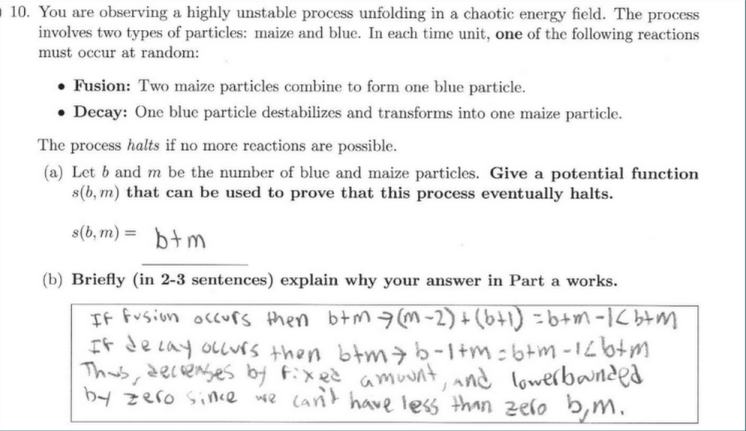
\includegraphics[scale=0.75]{Q10.png}
\end{center}
My solution was deficient because I forgot that the amount of maize particles decreased by one in the decay stage.

I could have fixed with the potential function $3b+2m$. Since if fusion then $3b+2m \to 3(b+1)+2(m-1)=3b+2m-1$ and if decay then $3b+2m \to 3(b-1)+2(m+1)=3b+2m-1$

\qh[Understanding $\mathsf{P}$, $\mathsf{NP}$, and $\mathsf{NP}$-hardness.]
\begin{subproblem}{}
    Prove that all efficiently decidable languages are efficiently verifiable. In other words, show that every language in $\mathsf{P}$ has an efficient verifier. 
\end{subproblem}
\begin{problemproof}
    Let $L \in \mathsf{P}$ thus there exists an efficient Turning Machine $M$ that decides $L$ in polynomial time.

    Let $V(x,c)=M(x)$.

    $V(x,c)$ is polynomial time since $M(x)$ is.

    If $x \in L$ then $M(x)$ accepts thus $V(x,c)$ accepts.

    If $x \notin L$ then $M(x)$ rejects thus $V(x,c)$ rejects for all $c$ since we ignore it.
\end{problemproof}

\begin{subproblem}{}
    Prove that every language in $\NP$ is decidable. In other words, show that every language in $\NP$ has a decider. 
\end{subproblem}
\begin{problemproof}
    Let $L \in \NP$ thus there exists an efficient verifier $V$ that is bounded by $p(|x|)$ a polynomial function.

    Define $M(x)=V(x,c)$ s.t. we loop over all strings $c$ s.t. $|c| \leq p(|x|)$ and accept if $V(x,c)$ accepts or reject if $V(x,c)$ rejects for all $c$.

    If $x  \in L$ then there exists a $c$ s.t. $p(|x|)\geq|c|$. Thus, our Turing machine $M(x)$ will loop through all possible strings $c$. Thus, eventually we will find a $c$ s.t. $V(x,c)$ accepts thus $M(x)$ accepts.

    If $x \notin L$ then there is no $c$ s.t. $p(|x|) \geq |c|$ s.t. $V(x,c)$ will accept. Thus, $M(x)$ will reject.

    Thus, $M$ is a decider for $L$. Thus, $\NP$ is a subset of decidable languages.
\end{problemproof}

\begin{subproblem}{}
    Prove or disprove: All $\NP$-hard languages are decidable. 

    (A disproof would consist of an $\NP$-hard language that is also undecidable.) 
\end{subproblem}
\begin{problemproof}
    False consider $L_{Halt}$. This is $\NP$-Hard by proven on discussion worksheet complexity and undecidable.
\end{problemproof}
\newcommand{\SubsetSum}{\textsc{SubsetSum}}
\begin{problem}{Verifying $\Upsilon$'s verifiers.}
    Recall that a \emph{multiset} $S$ is just like a set, but it can have duplicate elements. A submultiset $S^* \subseteq S$ also can have duplicate elements, as long as it does not have more copies of an particular element than $S$ does. 
    \[ 
        \SubsetSum = \{(S, k) : S \text{ is a \emph{multiset} of integers $\geq 0$, and } \exists\; S' \subseteq S \text{ such that } \sum_{s \in S'} s = k\}.
    \]
\end{problem}
\begin{subproblem}{}
    \begin{center}
      \begin{minipage}{0.9\linewidth}
        \begin{algorithm}[H]
       \begin{algorithmic}[1]
      \Require{A multiset of nonnegative integers $S = \{s_1, s_2, \ldots, s_n\}$, an integer $k$, and \emph{a multiset of nonnegative integers} $C = \{c_1, c_2, \ldots, c_m\}$}
         \Function{VerifierA}{$S, k, C$}
         \If{$m > n$} \textbf{reject} \Comment{$C$ can't be a submultiset of $S$ in this case} \EndIf 
         \State $sum \gets 0$
         \For{$c \in C$} \Comment{iterate over elements (integers) in $C$}
         \If{$c \notin S$} \textbf{reject} 
         \Else { $sum \gets sum + c$}
         \EndIf
         \EndFor
         \If {$sum = k$} \textbf{accept} \EndIf
         \State \textbf{reject}
         \EndFunction
       \end{algorithmic}
     \end{algorithm}  
     \end{minipage}
     \end{center}
    \begin{quote}
        \textbf{Correctness:} For correctness,
        \begin{align*}
            (S,k) \in \SubsetSum &\iff \text{there exists a submultiset $C \subseteq S$ s.t. $\sum_{c \in C} c = k$} \\
            & \iff \textsc{VerifierA}(S,k,C) \text{ accepts}
        \end{align*}
      
        \textbf{Runtime:} After ruling out the possibility that $m > n$ in line 2, the for loop will iterate over at most $n$ elements, while other lines take constant time, the overall runtime is $O(n)$, which is polynomial with respect to the input size. 
    \end{quote}

    Explain why \textsc{VerifierA} does not show that $\SubsetSum \in \NP$. You may use an example to support your reasoning. You do not have to fix the verifier, though it is a good exercise. 
\end{subproblem}
\vspace{10pt}
\begin{problemproof}
    \textsc{VerifierA} does not work since it does not account for if $C$ has more elements of one type then $S$. For example if $S=\{1,100,100,100,100\}$, $k=5$, and $C=\{1,1,1,1,1\}$. Then $V(S,k,C)$ would accept since $1 \in S$. Thus, $sum \leftarrow 5=k$, but $S$ cannot sum to $5$.
\end{problemproof}

\begin{subproblem}{}
    \begin{center}
      \begin{minipage}{0.9\linewidth}
        \begin{algorithm}[H]
       \begin{algorithmic}[1]
      \Require{A multiset of nonnegative integers $S = \{s_1, s_2, \ldots, s_n\}$, an integer $k$, and \emph{a collection of nonnegative integers multisets} $C = \{C_1, C_2, \ldots, C_m\}$}
         \Function{VerifierB}{$S, k, C$}
         \For{$C_i \in C$} \Comment{Iterate over multisets in $C$}
            \State Confirm that $C_i \subseteq S$
            \If {$\sum_{c \in C_i} = k$} \textbf{accept} \EndIf
         \EndFor
         \State \textbf{reject}
         \EndFunction
       \end{algorithmic}
     \end{algorithm}  
     \end{minipage}
     \end{center}

    \begin{quote}
        \textbf{Correctness:} For correctness,
        \begin{align*}
            (S,k) \in \SubsetSum &\iff \text{there exists a submultiset $C_i \subseteq S$ s.t. $\sum_{c \in C_i} c = k$} \\
            & \iff \text{there exists a collection $C$ that contains $C_i$}\\
            & \iff \textsc{VerifierB}(S,k,C) \text{ accepts}
        \end{align*}
      
        \textbf{Runtime:} In line 4, since $C_i$ is confirmed to be a submultiset of~$S$, $|C_i| \leq n$ and hence summing all items takes $O(n)$. Since there are $m$ sets in $C$, the overall runtime is $O(mn)$, which is polynomial with respect to the input size. 
    \end{quote}

      Explain why \textsc{VerifierB} does not show that $\SubsetSum \in \NP$. You may use an example to support your reasoning. You do not have to fix the verifier, though it is a good exercise. 
\end{subproblem}
\begin{problemproof}
    Consider $C=\{C_1,C_2\}$ s.t. $C_1 \subset S$ whose elements sum to $k$, and $C_2$ s.t. $|C_2|=|S|^4$. Thus, even though the certificate is correct $|C_2|$ is not a polynomial in $|S|$.
\end{problemproof}

\begin{subproblem}{}
    \begin{center}
        \begin{minipage}{0.9\linewidth}
          \begin{algorithm}[H]
         \begin{algorithmic}[1]
        \Require{A multiset of nonnegative integers $S = \{s_1, s_2, \ldots, s_n\}$, an integer $k$, and \emph{an array of bits} $C[1,\ldots,n]$}
           \Function{VerifierC}{$S, k, C$}
              \State $sum \gets 0$
              \For {$i = 1, \ldots, n$}
                  \If {$C[i] = 1$} $sum \gets sum + s_i$ \EndIf
              \EndFor
           \If {$sum = k$} \textbf{accept} \EndIf
           \State \textbf{reject}
           \EndFunction
         \end{algorithmic}
       \end{algorithm}  
       \end{minipage}
       \end{center}
  
       $\Upsilon$ claims that Lambda's verifier is incorrect with the following counterexample:
       \begin{quote}
           Consider $S = \{1,1,2,5\}$, $k = 7$, and $C=[0,1,0,1]$. Clearly, $S \in \SubsetSum$, but $1 + 5 =6 \neq 7$ so the verifier rejects. Therefore, \textsc{VerifierC} must be incorrect!
       \end{quote}
  
       Explain why $\Upsilon$'s claim is unfounded. 
\end{subproblem}
\begin{solution}
    This is unfounded since there exists $C=[0,0,1,1]$ s.t. $V(S,7,C)$ accepts. We cannot throw out a verifier if one $C$ does not work we have to check all $C$ of a certain size.
\end{solution}

\end{document}

